% This must be in the first 5 lines to tell arXiv to use pdfLaTeX, which is strongly recommended.
\pdfoutput=1
% In particular, the hyperref package requires pdfLaTeX in order to break URLs across lines.

\documentclass[11pt]{article}
% Change "review" to "final" to generate the final (sometimes called camera-ready) version.
% Change to "preprint" to generate a non-anonymous version with page numbers.
% \usepackage[review]{acl}
\usepackage{acl}

% Standard package includes
\usepackage{times}
\usepackage{latexsym}
\usepackage[T1]{fontenc}
\usepackage[utf8]{inputenc}
\usepackage{microtype}
\usepackage{inconsolata}
\usepackage{graphicx}
\usepackage{amsmath}
\usepackage{booktabs}
\usepackage{lipsum}
\usepackage[caption=false]{subfig}
\usepackage{float}
\usepackage{multirow}
\usepackage{amsmath}
\usepackage{changepage}

\DeclareMathOperator*{\argmax}{arg\,max}

\usepackage[]{todonotes}                                 % use option "disable" to suppress notes
\makeatletter
\newcommand*\iftodonotes{\if@todonotes@disabled\expandafter\@secondoftwo\else\expandafter\@firstoftwo\fi}  
\makeatother
\newcommand{\noindentaftertodo}{\iftodonotes{\noindent}{}\ignorespaces}

\newcommand{\response}[1]{\vspace{3pt}\hrule\vspace{3pt}\textbf{#1:}}

\interfootnotelinepenalty=10000


\title{A Pragmatic Approach to Non-Generic Summarization}

\author{
xxx Spinoso-Di Piano \\
McGill University \\
\texttt{xxx.spinoso-dipiano@mail.mcgill.ca}
}

\begin{document}

\maketitle

\begin{abstract}
    There has been growing interest in modeling the task of summarization through a pragmatic point of view by imagining what a reader might understand from a generated summary. This approach to summarization has been taken using the Rational Speech Acts (RSA) framework in which the goodness of a generated summary is determined by how well a reader might reconstruct the initial source document from the generated summary. However, in this paper, we argue that this \emph{source reconstruction} objective is unrealistic and is a symptom of the underspecified nature of \emph{generic} summarization. As a result, we move this pragmatic modeling focus away from generic summarization and towards \emph{non-generic summarization}, the task of generating a summary which meets some additional information request (e.g., providing the answer to a question). To use RSA in this setting, we introduce the \emph{latent reconstruction} objective which rescores candidate summaries based on a reader's ability to reconstruct the value of a latent variable related to the summary's information request. With this more realistic implementation of the intended meaning of a non-generic summary, we are able to achieve competitive ROUGE scores offering a path towards pragmatically modeling non-generic summarization.
\end{abstract}


\section{Introduction}

Automatic summarization is the computational task consisting of distilling the contents of a source document down to its most important parts. This task has seen growing interest in recent years with numerous publications contributing novel, often neural-based, approaches to both extractive and abstractive summarization \citep{rush-etal-2015-neural,nallapati-etal-2016-abstractive,see-etal-2017-get}. In particular, one recent line of work has focused on developing summarization systems which improve the informativeness of generated summaries by imagining what a reader might take away after reading a system-generated summary \citep{shen-etal-2019-pragmatically}. Intuitively, this focus on the reader's interpretation of the generated summary should force the summarization system to act more pragmatically e.g., by providing additional details for surprising or ambiguous information and by omitting details which should be understood from the context.

More formally, this pragmatic way of viewing summary generation is inspired by the Rational Speech Acts (RSA) framework \citep{degen_rational_2023}. In RSA, a speaker attempts to convey a piece of information to a listener by generating an utterance which the speaker believes will be easily and unambiguously understood by the listener. To do so, the speaker, often referred to as the pragmatic speaker, will generate an utterance $u$ where the intended meaning of the utterance $m$ is likely to be recovered by the listener, often referred to as the literal listener, when observing $u$. Translating this to the context of summarization, a pragmatic summarizer will, given a source text $x$, produce a summary $y$ for which a literal reader is likely to recover the summary's intended meaning $m$.

Although appealing in principle, existing approaches which embed the task of automatic summarization within RSA suffer from one common difficulty: implementing the intended meaning $m$ of a summary $y$. One existing approach approximates the recovery of the intended meaning as a source reconstruction objective \citep{shen-etal-2019-pragmatically}. That is, under the source-reconstruction-based meaning implementation, a good generated summary $y$ should allow a literal listener to easily reconstruct the source document $x$. Convenient as it may be, we do not believe source reconstruction to be a faithful approximation of recovering the intended meaning of a summary. For instance, a summarization system may correctly choose to drop unimportant information from the source text in the summary thereby making it virtually impossible to perfectly recover the source text from the generated summary.\todo{This intuition is similar to the LeCun paper. For instance, Figure 6 in that paper shows that the predictor has learned a higher-level semantic representation of patches and so can ``roughly'' reconstruct it.}

In fact, the difficulty of providing a suitable proxy for the intended meaning of a summary may be due to the inherently ill-defined nature of \emph{generic} summarization, the task of generating a summary from a source text without any additional specifications on the output summary (Figure~\ref{fig:example-generic-summ-llama}). Indeed, as \citet{kryscinski2019neural} argues, the task of generic summarization is underspecified since what information is included in a summary and, by extension, its intended meaning, depend on unspecified user preferences and information needs. Consequently, expecting a literal reader to recover the intended meaning of a summary which was, at the outset, unobserved by the summarizer may be an unattainable objective. Thus, due to its underspecification, generic summarization may not be an appropriate task for the RSA modeling framework and even, more generally, for a pragmatics-based modeling approach.

\begin{figure}[t]
    \centering
    \includegraphics[width=\linewidth]{figs/Slide1.PNG}
    \caption{An example of a \emph{generic summary} (truncated) for \href{https://www.cnn.com/2018/05/21/opinions/trump-investigation-order-twitter-opinion-callan/index.html}{\underline{this article}} from the MultiOpEd dataset (Section~\ref{sec:datasets}) generated by Llama2.}
    \label{fig:example-generic-summ-llama}
\end{figure}

As a result, in this paper, we re-focus the use of the RSA modeling framework to the task of \emph{non-generic} summarization, the task of generating a summary from a source text while meeting some additional information request. The advantage of this setting over generic summarization is that it specifies an additional input which could be helpful in formulating a more realistic proxy to a summary's intended meaning. For example, a non-generic summary of a news editorial might involve summarizing the article while answering a question related to it as illustrated in Figure~\ref{fig:example-non-generic-summ-llama}. In this case, we believe a realistic approximation of the intended meaning of a summary is providing an answer to the initial question about the news editorial. This example motivates the introduction of the \emph{latent reconstruction} objective whereby a good summary should allow the literal reader to easily reconstruct the value of some latent variable $Z$ related to the information request of the non-generic summary.

\begin{figure}[t]
    \centering
    \includegraphics[width=\linewidth]{figs/Slide2.PNG}
    \caption{An example of a \emph{non-generic summary} (truncated) generated by Llama2 for the same article as in Figure~\ref{fig:example-generic-summ-llama}. The question which was asked about this article ([QUESTION]) was ``Is Trump's investigation into the FBI justified?''}
    \label{fig:example-non-generic-summ-llama}
\end{figure}

We evaluate several summarization systems on multiple non-generic summarization datasets and find that the latent reconstruction is a competitive alternative to modeling non-generic summarization. In addition, we find that combining the latent and source reconstruction objectives together leads to performance gains over both reconstruction objectives used individually. This offers a new promising future direction in pragmatically improving non-generic summarization systems by balancing different meaning recovery objectives in the context of RSA.

To summarize, the research question we address in our work is ``Is a pragmatics-based approach to non-generic summarization a viable modeling approach?''. Or, more specifically, ``Can RSA, through the latent reconstruction objective, be used for non-generic summarization?''. To this end, the contributions of this paper are as follows:\todo{Jackie's comment: Well, what do you mean here? What is pragmatics-based and what do we mean by non-generic summarization?}

\begin{itemize}
    \item We provide a pragmatics-based perspective to modeling the task of non-generic summarization by using the RSA framework and approximating the intended meaning of the summary as the latent reconstruction objective.
    \item We compare against existing summarization methods and show that using RSA with the latent reconstruction objective offers a promising path towards pragmatically modeling non-generic summarization.
\end{itemize}

%

\section{Related Work}

\subsection{Non-generic summarization}

Several types of non-generic summarization tasks have already been studied. The most prominent one is the query-focused summarization (QFS) task in which a summary is generated from a single or multiple documents such that it can provide information related to a given query or queries \citep{dangDUC2005Evaluation2006,daumeBayesianQueryfocusedSummarization2006,suCAiRECOVIDQuestionAnswering2020,xuCoarsetoFineQueryFocused2020}. The query can be a collection of keywords, a question or a longer passage describing some information request. In addition to QFS, other forms of non-generic summarization tasks have attempted to tailor the generated summary to some specified user preference. For instance, previous studies have explored personalizing a summary based on a user's preferred summary length, style and interests \citep{fanControllableAbstractiveSummarization2018}, their preferences between lay and technical summaries \citep{tauchmannGenericSummarizationMultifaceted2018,shaibSummarizingSimplifyingSynthesizing2023a} as well as their news interests in the context of personalized news headlines generation \citep{aoPENSDatasetGeneric2021}.

There have been several proposed modeling approaches for non-generic summarization. In QFS, the two most common approaches have been a two-step retrieval-abstraction method and an end-to-end method \citep{vigExploringNeuralModels2022}. In other non-generic summarization tasks, studies have attempted to model user preferences either by creating representations for the preferences and injecting them into an encoder-decoder summarization model \citep{fanControllableAbstractiveSummarization2018,aoPENSDatasetGeneric2021} or, more recently, via prompt engineering and in-context learning \citep{shaibSummarizingSimplifyingSynthesizing2023a,yangExploringLimitsChatGPT2023}. To the best of our knowledge, there has not been a pragmatics-based approach to non-generic summarization.

\subsection{RSA for Language Generation}

The RSA framework has been used to model several language generation tasks in the hopes of introducing some of the pragmatics-based notions which make human communication so effective \citep{grice1975logic}. In \citet{andreasReasoningPragmaticsNeural2016}, the authors model the task of informative image captioning by using, for the first time, \emph{neural} listeners and speakers. \citet{cohn-gordonPragmaticallyInformativeImage2018a} offers to solve some of the inefficiencies of using RSA for image captioning by generating captions at the character level. \citet{friedUnifiedPragmaticModels2018} extend the use of RSA to instruction following and generation and \citet{see-etal-2017-get} investigate its use for generic summarization and for generation from structured data. More recently, \citet{Nie2020PragmaticII} develop an RSA model for issue-sensitive image captioning and \citet{Nguyen2023LanguageMA} try to characterize the behaviour of large language models (LLMs) by framing them in the context of the speaker-listener RSA model of communication. 

\section{RSA for Non-Generic Summarization}

\label{sec:rsa_for_nongen_summ}

We present our approach to modeling non-generic summarization via RSA by first discussing the general underlying principles of RSA and, subsequently, by discussing the extensions we propose to allow this framework to support the modeling of non-generic summarization.

In the RSA theory for modeling communication, a pragmatic speaker, $S_1$, attempts to convey a message with some meaning, $m$, by generating an utterance, $u$. To do so, the pragmatic speaker uses a \emph{literal speaker}, $S_0$, to first generate candidate utterances $\mathcal{U}$ where the utterances $u \in \mathcal{U}$ are generated from a uniform distribution, $P_{S_0}(U | M = m)$, over utterances with literal meaning matching $m$. The pragmatic speaker then re-scores each candidate utterance, $u \in \mathcal{U}$, by using the probability that a literal listener, $L_0$, recovers the intended meaning of their message by observing $u$, $P_{L_0}(M = m | U = u)$. Finally, the pragmatic speaker combines these two probabilities with a rationality parameter $\lambda$ to provide a final score for each utterance $u \in \mathcal{U}$ represented by\footnote{We drop the $P_{S_1}$ notation for the pragmatic speaker as, except for $\lambda = 0,1$, this product does not necessarily induce a valid probability distribution.}

\begin{equation}
    S_1(u|m) = P_{S_0}(u|m)^\lambda \cdot P_{L_0}(m|u)^{1 - \lambda}
\end{equation}

To adapt the RSA model to the task of non-generic summarization, we provide new definitions for the speakers, $S_0,S_1$, and listener, $L_0$, which we refer to as summarizers, $S_0,S_1$, and readers, $R_0$, respectively. We define the literal summarizer as a base summarization system, $P_{S_0}(Y|X = x, R = r)$, which takes as input some source text $x$ and information request $r$. To define the literal reader, we approximate the recovery of the intended meaning of a summary $y$ through the \emph{latent reconstruction} objective. In this reconstruction objective, we use a language model conditioned on $y$ with reconstruction target being the value $z$ of a latent variable $Z$ related to the initial information request $r$, $P_{R_0}(z | y)$. This latent reconstruction objective is then used by the pragmatic summarizer, $S_1$, to provide a final score to a summary $y$

\begin{equation}
    \label{eqn:prag_summ}
    S_1(y|x) = P_{S_0}(y|x,r)^\lambda \cdot P_{R_0}(z|y)^{1 - \lambda}
\end{equation}

The latent reconstruction objective is, to the best of our knowledge, the first implementation of the intended meaning of a non-generic summary in the context of RSA. Previous approaches in generic summarization have included the source reconstruction objective where the reconstruction target is the source text $x$ as well as the distractor-based objective where, given a generic summary, $y$, $R_0$ should distinguish between the true source text $x$ and a distractor source text $x'$ \citep{andreasReasoningPragmaticsNeural2016,cohn-gordonPragmaticallyInformativeImage2018a, see-etal-2017-get}. We believe that, in the context of non-generic summarization, the latent reconstruction objective is more in line with the true intended meaning of a summary than previous implementations of meaning in generic summarization.

\section{Experiments}

In this section, we describe the experiments, datasets and evaluations we use to verify our hypothesis that a viable approach to non-generic summarization via RSA involves the latent reconstruction objective presented in Section~\ref{sec:rsa_for_nongen_summ}.

\subsection{Experimental Setup}

We describe the pieces of our RSA-based non-generic summarization pipeline which starts with candidate summary generations by the literal summarizer, then goes through summary rescoring by the literal reader and final summary selection by the pragmatic summarizer.

\subsubsection{Literal Summarizers}

We use different pre-trained summarization systems as literal summarizers in our RSA setup of non-generic summarization. For each source text-information request pair, we use each summarization system to produce 5 candidate summaries using diverse beam search \citep{diverse_beam_search} (DBS). DBS is a variant of beam search which optimizes its decoding step for a diversity-augmented objective. We briefly describe the different summarization systems below. All model checkpoints are taken from HuggingFace \footnote{\url{https://huggingface.co/}}.

\paragraph{BART} BART \citep{bart_model} is an encoder-decoder Transformer model trained with a denoising objective function and commonly used for language generation tasks. We use the \texttt{facebook/bart-large-cnn} checkpoint of BART which is fine-tuned on the CNN/Daily Mail summarization dataset. To account for the additional information request, we follow previous query-focused summarization work \citep{vigExploringNeuralModels2022} and preprocess the input to BART by concatenating the information request and the source text with the model's delimiter token. We truncate the input from the right so that it fits within BART's 1024 maximum input token limit.

\paragraph{LED} Similar to BART, the Longformer Encoder-Decoder \citep{longformer_conditional} (LED) is an auto-denoising encoder-decoder which uses a Longformer as its encoder. The Longformer encoder uses a memory-efficient version of attention to allow for a maximum input token limit of 16384 tokens which may be beneficial in cases where the source text exceeds BART's 1024 input token limit. We use the \texttt{allenai/led-large-16384-arxiv} checkpoint of LED which is fine-tuned on the arXiv scientific article summarization dataset. We use the same input preprocessing decision as for BART to account for the additional information request of the non-generic summaries. 

\paragraph{LLama2} Llama2 \citep{touvronLlamaOpenFoundation2023} is a collection of LLMs developed by Meta pre-trained and fine-tuned on a ``mix of publicly available online data.'' This class of models has been shown to be competitive on some summarization benchmarks \citep{yangExploringLimitsChatGPT2023,zhangBenchmarkingLargeLanguage2024}. We use the \texttt{meta-llama/Llama-2-7b-chat-hf} checkpoint which is the 7 billion parameter version of Llama2 fine-tuned with both instruction tuning and reinforcement learning from human feedback (RLHF). We use the prompt shown in Figure~\ref{fig:example-non-generic-summ-llama} for non-generic summarization where the [QUESTION] placeholder is replaced by the information request.

\subsubsection{Literal Reader}

To implement the literal reader, we use the \texttt{google/flan-t5-large} checkpoint of the FLAN-T5 \citep{chung2022scaling} series of general purpose LLMs. The FLAN-T5 LLM series is a collection of large language models with the same architecture as the original T5 series but trained on additional tasks and fine-tuned with instruction tuning. We use the large (700 million parameters) version as a compromise between inference speed and capacity.

\subsubsection{Pragmatic Summarizer}

The pragmatic summarizer combines the likelihood scores produced by the summarization system and the LLM to select the final summary from the pool of 5 candidate summaries i.e., the final selected summary is
\begin{equation}    
    \argmax_{i=1 \dots 5} P_{S_0}(\hat{y}_i|x,r)^\lambda \cdot P_{R_0}(z|\hat{y}_i)^{1 - \lambda}
\end{equation}
for some $\lambda \in [0, 1]$.

\subsection{Datasets}

\label{sec:datasets}

In this section, we describe the datasets that we use to run our experiments on the different implementations of $S_0, S_1, R_0$ in the context of non-generic summarization. We also describe our choice of information request and latent variable for each dataset. In addition, we provide examples of the different types of source texts, information requests and latent variables in Table~\ref{tab:summ_examples} and summary statistics for each dataset in Table~\ref{tab:summ_stats}.

\begin{table*}[t]
\centering
\resizebox{\linewidth}{!}{
\begin{tabular}{lp{10cm}p{4cm}p{3cm}}
\toprule
Dataset Name & Source text & Information request & Latent variable \\
\midrule
CovidET & I dont even know how to speak of this grief. I have read of many stories of people losing their loved ones, but it didnt happen to [...] & Describe the disgust of this post & Disgust \\
Debatepedia & [...] Inviting foreigners to come to america as guest workers is equivalent to sending the message : you people are only fit to do menial jobs that americans think they are too good to do [...] & Would a guest worker program be fair to guest workers? & Guest workers \\
DUC 2007 & In February 1999 some of OJ Simpson's possessions including his Heisman Trophy were sold at an auction which raised about \$430,000.  The proceeds were to go to the Brown [...] & Give an account of the developments in the life of OJ Simpson. & OJ Simpson developments \\
MultiOpEd & [...] Early Sunday afternoon President Donald Trump elevated Twitter to a virtual Cabinet position in his administration. He used it, rather than the attorney general, to order a possible criminal [...] & Is trump's investigation into the FBI justified? & Trump's trying to smear the Russia probe \\
QMSum & PhD F : We um \{disfmarker\} So we just put in an order for about twelve new machines, uh, to use as sort of a compute farm.  And um, uh, we ordered uh, SUN - Blade - one - hundreds, [...] & What did PhD F think about computational resources? & - \\
\bottomrule
\end{tabular}
}
\caption{Examples of source texts (truncated) along with their corresponding information request and latent variable for each dataset we use. We omit the latent variable for QMSum since it is the same as its information request.}
\label{tab:summ_examples}
\end{table*}

\begin{table}[t]
    \centering
    \resizebox{\linewidth}{!}{
    \begin{tabular}{lccccc}
        \toprule
         \multirow{3}{*}{\begin{tabular}{@{}l@{}}Dataset \\ Name\end{tabular}} & \multirow{3}{*}{\begin{tabular}{@{}l@{}}Test \\ Size\end{tabular}} & \multicolumn{4}{c}{Average length} \\
        & & Source & \begin{tabular}{@{}c@{}}Information \\ Request\end{tabular} & \begin{tabular}{@{}c@{}} Latent \\ Variable \end{tabular} & \begin{tabular}{@{}c@{}} Reference \\ Summary \end{tabular} \\
        \cmidrule{3-6}
        CovidET & 1043 & 171 & 6 & 1 & 22 \\
        Debatepedia & 893 & 70 & 9 & 1 & 10 \\
        DUC 2007 & 1124 & 466 & 22 & 4 & 243 \\
        MultiOpEd & 531 & 925 & 7 & 7 & 102 \\
        QMSum & 244 & 1020 & 13 & 13 & 58 \\
        \bottomrule
    \end{tabular}
    }
    \caption{Summary statistics for each of the datasets. Test size refers to the number of unique source text-information request pairs in the test set of each dataset and the average length refers to the average space-separated string lengths of different dataset fields.}
    \label{tab:summ_stats}
\end{table}

\paragraph{CovidET} The CovidET dataset \citep{zhan-etal-2022-feel} is a collection of Reddit\footnote{\url{https://www.reddit.com/}} posts about different personal events experienced by people during the Covid-19 pandemic. Each post has multiple human-written reference summaries which each summarize one of the different emotions found in the Reddit post as well as the emotion's associated cause(s) or trigger(s).

In the case of CovidET, no information request is explicitly provided, thus we take the emotion $e$ being summarized and convert it to the instruction ``Describe the $e$ of this post.'' to make an information request. We use the emotion $e$ as the latent variable.

\paragraph{Debatepedia} The Debatepedia dataset \citep{nema-etal-2017-diversity} is a collection of argumentative texts with a for or against stance related to a certain topic (e.g., politics, crime, environment, etc.). Each text has a certain topic and question associated with it, with certain texts having multiple associated topic-question pairs. Each text and topic-question pair has a human-written reference summary which summarizes the text by providing an answer to its related question.

For Debatepedia, we use the question associated with the source text as the summary's information request and the topic of the question as the latent variable.

\paragraph{DUC 2007}  The DUC 2007 dataset \citep{duc2007} is a multi-document query-focused summarization dataset with source texts consisting of news articles from the Associated Press, the New York Times (1998-2000) and the Xinhua News Agency (1996-2000). The news articles are grouped into collections of 25 news articles, all covering the same topic. A question is then associated with each group of 25 news articles and 4 human-written reference summaries are produced summarizing the 25 news articles while answering the initial question. Because handling multiple documents is beyond the scope of this work, we associate each topic, question and reference summaries with each of their corresponding 25 news articles to create a single-document non-generic summarization dataset.

Similar to Debatepedia, we use the question as the information request and the topic of the question as the latent variable.

\paragraph{MultiOpEd} The MultiOpEd dataset \citep{liu-etal-2021-multioped} is a collection of news editorials which provide a perspective on a certain question about a controversial topic. The news editorial is accompanied by an abstract summarizing its stance and arguments and a perspective which provides a concise answer to the initial question.

For MultiOpEd, we use the question being asked as the information request and the perspective as the latent variable.

\paragraph{QMSum} The QMSum dataset \citep{qmsum} is a query-focused meeting summarization dataset where the source texts are excerpts from different meeting transcripts. Each excerpt has an associated question and reference summary summarizing the excerpt while providing an answer to the question.

In the case of QMSum, we use the question being asked about the meeting transcript excerpt as the information request. Since no answers to questions are explicitly provided in the dataset, we assume that the latent variable is the same as the summary's information request.

\subsection{Evaluation}

We evaluate our non-generic summarization pipeline by computing the ROUGE-1, ROUGE-2 and ROUGE-L scores between the summary selected by the pragmatic summarizer and the reference summary. In the case that several reference summaries have been written for the same source text-information request pair (e.g., DUC 2007), we take the maximum ROUGE scores.

\section{Results and Analysis}

In this section, we present the results and analyses of our experiments which test the viability of using different variants of pragmatic summarizers in the context of modeling non-generic summarization via RSA.

\subsection{Reconstruction-Only $S_1$}

\label{sec:prbs}

\begin{table*}
\centering
    \resizebox{0.75\linewidth}{!}{
        \begin{tabular}{lccccccccc}
        \toprule
        & \multicolumn{3}{c}{BART} & \multicolumn{3}{c}{LED} & \multicolumn{3}{c}{Llama2} \\
        \cmidrule(r){2-4}\cmidrule(r){5-7}\cmidrule(r){8-10}
        & R-1 & R-2 & R-L & R-1 & R-2 & R-L & R-1 & R-2 & R-L \\
        \midrule
        Random &                 0.257      & 0.049         & 0.153         &  0.251 & 0.040 & 0.146  &  \bf 0.322 & \bf 0.070 & \bf 0.176 \\
        $P_{S_0}(\hat{y} | x)$ & 0.260      & 0.047         & 0.152         &  0.219 & 0.038 & 0.127  &  0.321 & 0.069 & 0.175 \\
        $P_{R_0}(x | \hat{y})$ & 0.257      & 0.048         & 0.150         &  \bf 0.288 & \bf 0.047 & \bf 0.154  &  0.318 & 0.069 & 0.172 \\
        $P_{R_0}(z | \hat{y})$ & \bf 0.267  & \bf 0.053     & \bf 0.156    &  0.242 & 0.043 & 0.138  &  0.320 & 0.069 & 0.174 \\
        \midrule 
        Oracle &                 0.297      & 0.071         & 0.178         &  0.320 & 0.066 & 0.180  &  0.355 & 0.089 & 0.197 \\
        \midrule
        SOTA & \multicolumn{9}{c}{0.315/0.138/0.298 \citep{Xu2023LMGQSAL}} \\
        \bottomrule
        \end{tabular}
    }
\caption{ROUGE scores for the reconstruction-only $S_1$ setting described in Section~\ref{sec:prbs} on the MultiOpEd dataset. We also include the ROUGE scores of the existing state-of-the-art (SOTA) non-generic summarization model on this dataset.}
\label{tab:multioped}
\end{table*}

\begin{table*}
\centering
    \resizebox{0.75\linewidth}{!}{
        \begin{tabular}{lccccccccc}
        \toprule
        & \multicolumn{3}{c}{BART} & \multicolumn{3}{c}{LED} & \multicolumn{3}{c}{Llama2} \\
        Dataset & R-1 & R-2 & R-L & R-1 & R-2 & R-L & R-1 & R-2 & R-L \\
        \cmidrule(r){2-4}\cmidrule(r){5-7}\cmidrule(r){8-10}
 CovidET     & $+$2.24           & $+$3.66           & $+$4.08           & $-$16.42         & $-$18.90         & $-$13.25         & $+$0.55             & $+$0.52             & $+$1.93             \\
 Debatepedia & $-$0.80           & $+$0.77           & $-$0.23           & $-$6.63          & $-$8.13          & $-$5.08          & $-$5.60             & $-$9.85             & $-$5.34             \\
 DUC 2007  & $+$0.35           & $+$4.24           & $+$2.14           & $-$8.45          & $-$5.52          & $-$5.02          & $+$0.74             & $+$0.90             & $+$0.70             \\
 MultiOpEd   & $+$3.74           & $+$11.11          & $+$4.23           & $-$15.94         & $-$7.64          & $-$10.56         & $+$0.70             & $+$0.99             & $+$1.03             \\
 QMSum       & $+$4.71           & $+$3.53           & $+$4.87           & $-$5.04          & $-$5.90          & $-$1.06          & $-$0.09             & $-$0.65             & $-$1.01             \\
        \bottomrule
        \end{tabular}
    }
\caption{Relative average ROUGE score performance differences between a pragmatic summarizer which uses the latent reconstruction objective and one that uses the source reconstruction objective. A value of $+x$ implies that the average ROUGE score achieved with the latent reconstruction objective is $x\%$ higher than the one achieved with the source reconstruction objective.}
\label{table:relative_latent_source}
\end{table*}

\begin{table}
\centering
    \resizebox{\linewidth}{!}{
        \begin{tabular}{lcccccc}
        \toprule
        & \multicolumn{2}{c}{R-1} & \multicolumn{2}{c}{R-2} & \multicolumn{2}{c}{R-L}  \\
        & Freq. & $\%$ & Freq. & $\%$ & Freq. & $\%$ \\
        \cmidrule(r){2-3} \cmidrule(r){4-5} \cmidrule(r){6-7}
        Random &                 2 & 13.3 & 2 & 13.3 & 2 & 13.3 \\
        $P_{S_0}(\hat{y} | x)$ & 2 & 13.3 & 4 & 26.7 & 2 & 13.3 \\
        $P_{R_0}(x | \hat{y})$ & 6 & 40.0 & 6 & 40.0 & 6 & 40.0 \\
        $P_{R_0}(z | \hat{y})$ & 5 & 33.3 & 3 & 20.0 & 5 & 33.3 \\
        \bottomrule
        \end{tabular}
    }
\caption{Frequencies for when the maximal ROUGE score is achieved by the different models described in Section~\ref{sec:prbs}. The frequencies are computed across all datasets and for every literal summarizer implementation.}
\label{tab:battle_direct_rec}
\end{table}


We first present the results for what we call the reconstruction-only pragmatic summarizer in which we set the rationality parameter value to $\lambda = 0$. In the case of $\lambda = 0$, the pragmatic summarizer selects the final summary uniquely based on $P_{R_0}(z|\hat{y})$ (Equation~\ref{eqn:prag_summ}). To understand the usefulness of the latent reconstruction objective, we implement an additional pragmatic speaker which uses the source reconstruction objective in its scoring function with $\lambda = 0$. Additionally, we compare the reconstruction-only $S_1$'s with the setting where $\lambda = 1$ i.e., where the summary selected by $S_1$ is the one with the highest likelihood score according to the literal summarizer, $S_0$. Finally, we also implement a Random baseline where the final summary is selected at random and an Oracle upper-bound which selects the candidate summary which maximizes the ROUGE score with the reference summary(ies). The results for the MultiOpEd dataset are presented in Table~\ref{tab:multioped} and the results for the other datasets can be found in Appendix~\ref{sec:app_add_results_prbs}.

We observe that, across all datasets and all literal summarizers, a reconstruction-only pragmatic summarizer, via either the latent or the source reconstruction objective, is likely to lead to higher ROUGE scores than relying on the initial likelihood scores of the literal summarizer. This finding is illustrated through Table~\ref{tab:battle_direct_rec} which aggregates the ROUGE performance scores from Table~\ref{tab:multioped} and Appendix~\ref{sec:app_add_results_prbs} by counting, for each dataset and each literal summarizer, which final summary selection method achieves the highest ROUGE score.

In terms of determining which of the reconstruction objectives is more suitable for non-generic summarization, the frequencies provided by Table~\ref{tab:battle_direct_rec} do not provide decisive evidence. As a result, to further compare these two reconstruction objectives, we compute the relative ROUGE score performance difference between using the latent reconstruction objective and the source reconstruction objective in the pragmatic summarizer's scoring function. These relative score differences can be found in Table~\ref{table:relative_latent_source}. Although it appears that the latent reconstruction objective is always detrimental for the LED literal summarizer, it appears to be beneficial in most cases when the literal summarizer is either BART of LLama2. These results offer a promising case for using the latent reconstruction objective to implement meaning in the RSA framework when modeling non-generic summarization.

Despite promising results, the method of selecting final summaries using the latent reconstruction objective and a rationality parameter value of $\lambda = 0$ remains sub-optimal when comparing its ROUGE scores to the ones achieved by the Oracle upper-bound. These relative performance differences are presented in Table~\ref{tab:relative_oracle} of Appendix~\ref{sec:app_add_results_prbs} and motivate the exploration of pragmatic speaker variants where $\lambda  \in (0,1)$.

\subsection{Rationality Parameter Interpolation}

To further investigate the viability of the latent reconstruction objective for modeling non-generic summarization via RSA, we evaluate the performance of pragmatic summarizers when the rationality parameter $\lambda$ from Equation~\ref{eqn:prag_summ} varies from 0 to 1. In particular, we compute the ROUGE scores for the final summaries selected by $S_1$ based on values of $\lambda \in [0, 0.1, \dots, 0.9, 1.0]$. We show a plot of ROUGE-1 scores for the pragmatic summarizer using the latent-reconstruction-based literal reader as well as the source-reconstruction-based literal reader in Figure~\ref{fig:line_plot}.

By analyzing the plots for every dataset and for every literal summarizer, we conclude that a rationality parameter which interpolates between the scores of the literal summarizer and the literal reader is more beneficial under the latent reconstruction objective than the source reconstruction objective. As Table~\ref{tab:battle_interpole} demonstrates, the highest attained ROUGE scores when using the latent reconstruction objective often occur for intermediate values of $\lambda \in (0,1)$. For the pragmatic summarizer which uses the source reconstruction objective, the highest ROUGE scores occur more commonly when the selection of the final summary is based only on the literal summarizer's score ($\lambda = 1$) or on the literal reader's score ($\lambda = 0$). This finding suggests that the latent reconstruction objective may be more appropriate in non-generic summarization as it forces the pragmatic summarizer to find a middle ground between overfitting to either the literal summarizer's or the literal reader's summary scores.

\begin{figure}
    \centering
    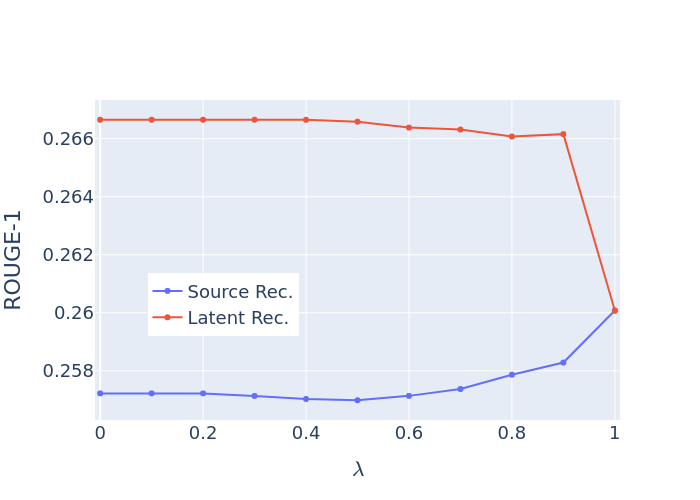
\includegraphics[width=\linewidth]{figs/rsa_lineplot_multioped_rouge1.png}
    \caption{Plot of the average ROUGE-1 scores for the summaries selected by a pragmatic summarizer using a latent reconstruction objective as well as a source reconstruction objective. In this case, the dataset is MultiOpEd and the literal summarizer used to generated the summaries is BART.}
    \label{fig:line_plot}
\end{figure}

\begin{table}
\begin{adjustwidth}{-2cm}{}
\centering
    \resizebox{\linewidth}{!}{
        \begin{tabular}{lcccccccccccc}
        \toprule
        & \multicolumn{6}{c}{Source Reconstruction} & \multicolumn{6}{c}{Latent Reconstruction}  \\
        \cmidrule(r){2-7} \cmidrule(r){8-13}
        & \multicolumn{2}{c}{R-1} & \multicolumn{2}{c}{R-2} & \multicolumn{2}{c}{R-L} & \multicolumn{2}{c}{R-1} & \multicolumn{2}{c}{R-2} & \multicolumn{2}{c}{R-L} \\
        & Freq. & $\%$ & Freq. & $\%$ & Freq. & $\%$ & Freq. & $\%$ & Freq. & $\%$ & Freq. & $\%$ \\
        \cmidrule(r){2-3} \cmidrule(r){4-5} \cmidrule(r){6-7} \cmidrule(r){8-9} \cmidrule(r){10-11} \cmidrule(r){12-13} 
        $\lambda = 0$           & 6 & 40.0 & 7 & 43.75 & 7 & 46.67 & 7 & 43.75 & 5 & 31.25 & 6 & 37.5 \\
        $\lambda \in (0, 1)$    & 2 & 13.33 & 6 & 37.50 & 1 & 6.67 & 5 & 31.25 & 7 & 43.75 & 8 & 50\\
    $\lambda = 1$               & 7 & 46.67 & 3 & 18.75 & 7 & 46.67 & 4 & 25.0 & 4 & 25.0 & 2 & 12.5 \\
        \bottomrule
        \end{tabular}
    }
\caption{Frequencies for when the maximum ROUGE score is achieved by the pragmatic summarizer using either the source or latent reconstruction objective and either $\lambda = 0$, $\lambda \in (0,1)$ or $\lambda = 1$.}
\label{tab:battle_interpole}
\end{adjustwidth}
\end{table}

\subsection{Latent-Source Reconstruction Objective}

Given the promise of interpolating the rationality parameter, we introduce another pragmatic summarizer which uses a hybrid latent-source reconstruction objective. To do so, we introduce a latent-source parameter $\alpha \in [0,1]$ which interpolates between the latent and source reconstruction objective. The pragmatic summarizer scoring function thus becomes
\begin{adjustwidth}{-2cm}{}
\begin{equation}
    S_1(y|x) = P_{S_0}(y|x,r)^\lambda \cdot \left ( P_{R_0}(x|y)^\alpha \cdot P_{R_0}(z|y)^{1 - \alpha}\right )^{1 - \lambda}
\end{equation}
\end{adjustwidth}

where we notice that for $\alpha = 0$ and $\alpha = 1$ we recover $S_1$'s scoring function using the latent and source reconstruction objectives respectively. For each dataset and for each literal summarizer, we compute the pragmatic summarizer's average ROUGE scores for every $\lambda \in [0, 0.1, \dots, 0.9, 1]$ and for every $\alpha \in [0, 0.1, \dots, 0.9, 1]$. A heatmap for the ROUGE-1 score on the MultiOpEd dataset using the BART literal summarizer is shown in Figure~\ref{fig:heatmap}.

By computing frequencies across all datasets and all literal summarizers, we observe that in most cases an intermediate value for both $\lambda \in (0,1)$ and $\alpha \in (0,1)$ is beneficial in terms of average ROUGE score (Table~\ref{tab:battle_all_interpole}). This finding suggests that the source reconstruction objective may hold additional signal which is orthogonal in terms of performance contribution to the latent reconstruction objective. This result may in part be due to the little information provided by the latent variables of most of the datasets we use. For instance, in the cases of CovidET and Debatepedia the value of the latent variables are typically one word and one noun phrase respectively.  In brief, the latent reconstruction objective may be the most beneficial in the context of non-generic summarization when paired with the source reconstruction objective.

\begin{figure}
    \centering
    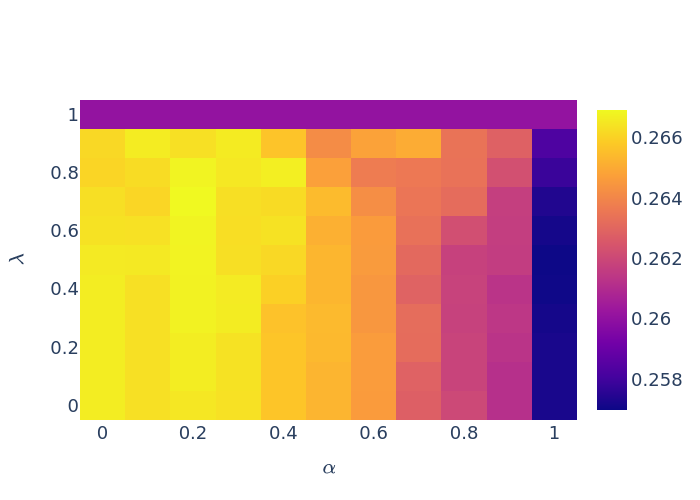
\includegraphics[width=\linewidth]{figs/rsa_weighted_multioped_rouge1.png}
    \caption{Heatmap of ROUGE-1 scores for different values of $\lambda$ and $\alpha$ on the MultiOpEd dataset using BART as the literal summarizer.}
    \label{fig:heatmap}
\end{figure}

\begin{table}
\centering
    \resizebox{\linewidth}{!}{
        \begin{tabular}{lcccccc}
        \toprule
        & \multicolumn{2}{c}{R-1} & \multicolumn{2}{c}{R-2} & \multicolumn{2}{c}{R-L}  \\
        & Freq. & $\%$ & Freq. & $\%$ & Freq. & $\%$ \\
        \cmidrule(r){2-3} \cmidrule(r){4-5} \cmidrule(r){6-7}
        $\lambda=1$ &           1 & 6.67 & 1 & 3.67 & 0 & 0.0 \\
        $\lambda=0,\alpha=1$ &  5 & 33.3 & 2 & 13.3 & 4 & 26.7 \\
        $\lambda=0,\alpha=0$ &  0 & 0.0 & 0 & 0.0 & 1 & 6.67 \\
        $\lambda \in (0, 1), \alpha \in (0, 1)$ &                 9 & 60.0 & 12 & 80.0 & 10 & 66.7 \\
        \bottomrule
        \end{tabular}
    }
\caption{Frequencies for when the maximum ROUGE score is achieved by the pragmatic summarizer using the latent-source reconstruction objective.}
\label{tab:battle_all_interpole}
\end{table}

\section{Conclusion}

In this paper, we have argued that previous attempts to model generic summarization via RSA have been inappropriate due to the infeasibility of the source reconstruction objective. As a result, we have argued for shifting the use of RSA to the context of non-generic summarization where the latent reconstruction objective is a more appropriate implementation of meaning. Through our experiments, we have shown that using the latent reconstruction objective in a pragmatic summarizer's scoring function may lead to performance improvements over existing summarization systems as well as over previous meaning implementations such as the source reconstruction objective. Furthermore, we find that the latent reconstruction objective may be most beneficial when paired with the source reconstruction objective as results suggest that these objectives offer complimentary information to the pragmatic summarizer. Thus, future work may investigate how these meaning implementations interact and whether they can be more seamlessly integrated within a non-generic summarization system which focuses on pragmatic language generation.

\section*{Limitations}

Despite our best efforts, this work suffers from shortcomings which prevent us from making more significant conclusions regarding the use of RSA and the latent reconstruction objective in non-generic summarization. Firstly, we do not explore the use of literal summarizers \emph{fine-tuned} on the datasets with which we experiment in this work. These fine-tuned models are responsible for achieving the existing SOTA ROUGE scores we presented in Table~\ref{tab:multioped} and in Appendix~\ref{sec:app_add_results_prbs}. This investigation is important since it is possible that when literal summarizers are fine-tuned there is no need for additional levels of reasoning as described in the RSA framework. Secondly, our exploration of alternative meaning implementations is limited to the source reconstruction objective and to the rescoring of 5 candidate summaries. A decoding method as described in \citet{cohn-gordonPragmaticallyInformativeImage2018a} which ``folds'' the reconstruction objective within its decoding step should also be compared against. Finally, in this work, we consider reconstruction objectives purely on the output space. However, a reconstruction objective in the representation space as described by \citet{assran2023selfsupervised} may be more suitable as it would not suffer from the lack of informativeness found in the latent variables we consider in this work.

\bibliography{custom}

\clearpage

\appendix

\onecolumn

\section{Additional Results}

\label{sec:app_add_results}

In this section, we provide additional results for all our experiments.

\subsection{Reconstruction-Only $S_1$}

\label{sec:app_add_results_prbs}

\begin{table}[H]
\centering
    \resizebox{0.75\linewidth}{!}{
        \begin{tabular}{lccccccccc}
        \toprule
         & \multicolumn{9}{c}{$S_0$} \\
         \cmidrule{2-10}
        & \multicolumn{3}{c}{BART} & \multicolumn{3}{c}{LED} & \multicolumn{3}{c}{Llama2} \\
        $R_0$ & R-1 & R-2 & R-L & R-1 & R-2 & R-L & R-1 & R-2 & R-L \\
        \cmidrule(r){2-4}\cmidrule(r){5-7}\cmidrule(r){8-10}
        Random &                 0.192 & 0.037 & 0.132 & 0.125 & 0.018 & 0.095 & \textbf{0.131} & \textbf{0.026} & \textbf{0.093} \\
        $P_{S_0}(\hat{y} | x)$ & 0.200 & 0.039 & 0.134 & 0.106 & 0.017 & 0.082 & 0.130 & \textbf{0.026} & 0.092 \\
        $P_{R_0}(x | \hat{y})$ & 0.199 & 0.039 & 0.133 & \textbf{0.150} &\textbf{ 0.025 }& \textbf{0.109} & 0.130 & \textbf{0.026} & 0.091 \\
        $P_{R_0}(z | \hat{y})$ & \textbf{0.204} & \textbf{0.041} & \textbf{0.139} & 0.125 & 0.020 & 0.094 & \textbf{0.131} & \textbf{0.026} & \textbf{0.093} \\
        \midrule 
        Oracle &                0.237 & 0.058 & 0.165 & 0.202 & 0.043 & 0.152 & 0.158 & 0.040 & 0.114 \\
        \midrule
        SOTA & \multicolumn{9}{c}{0.262/0.069/0.179 \citep{Yang2023ExploringTL}} \\
        \bottomrule
        \end{tabular}
    }
        \caption{ROUGE scores for the reconstruction-only $S_1$ setting described in Section~\ref{sec:prbs} on the CovidET dataset. We also include the ROUGE scores of the existing state-of-the-art (SOTA) non-generic summarization model on this dataset.}
\end{table}


\begin{table}[H]
\centering
    \resizebox{0.75\linewidth}{!}{
        \begin{tabular}{lccccccccc}
        \toprule
         & \multicolumn{9}{c}{$S_0$} \\
         \cmidrule{2-10}
        & \multicolumn{3}{c}{BART} & \multicolumn{3}{c}{LED} & \multicolumn{3}{c}{Llama2} \\
        $R_0$ & R-1 & R-2 & R-L & R-1 & R-2 & R-L & R-1 & R-2 & R-L \\
        \cmidrule(r){2-4}\cmidrule(r){5-7}\cmidrule(r){8-10}
        Random &                 0.144 & 0.045 & 0.120 & 0.079 & 0.022 & 0.071 & 0.080 & 0.024 & 0.069 \\
        $P_{S_0}(\hat{y} | x)$ & \textbf{0.147} & \textbf{0.046} & \textbf{0.121} & 0.075 & 0.022 & 0.067 & 0.079 & 0.023 & 0.068 \\
        $P_{R_0}(x | \hat{y})$ & 0.146 & 0.045 & 0.120 & \textbf{0.089} & \textbf{0.027} & \textbf{0.079} & \textbf{0.083} & \textbf{0.025} & \textbf{0.071} \\
        $P_{R_0}(z | \hat{y})$ & 0.145 & 0.045 & 0.120 & 0.083 & 0.025 & 0.075 & 0.078 & 0.023 & 0.067 \\
        \midrule 
        Oracle &                0.175 & 0.063 & 0.149 & 0.125 & 0.044 & 0.112 & 0.106 & 0.037 & 0.091 \\
        \midrule
        SOTA & \multicolumn{9}{c}{0.236/0.076/0.210 \citep{Xu2023LMGQSAL}} \\
        \bottomrule
        \end{tabular}
    }
        \caption{ROUGE scores for the reconstruction-only $S_1$ setting described in Section~\ref{sec:prbs} on the Debatepedia dataset. We also include the ROUGE scores of the existing state-of-the-art (SOTA) non-generic summarization model on this dataset.}
\end{table}


\begin{table}[H]
\centering
    \resizebox{0.75\linewidth}{!}{
        \begin{tabular}{lccccccccc}
        \toprule
         & \multicolumn{9}{c}{$S_0$} \\
         \cmidrule{2-10}
        & \multicolumn{3}{c}{BART} & \multicolumn{3}{c}{LED} & \multicolumn{3}{c}{Llama2} \\
        $R_0$ & R-1 & R-2 & R-L & R-1 & R-2 & R-L & R-1 & R-2 & R-L \\
        \cmidrule(r){2-4}\cmidrule(r){5-7}\cmidrule(r){8-10}
        Random &                 0.169 & 0.047 & 0.108 & 0.238 & 0.056 & 0.139 & 0.367 & 0.096 & 0.187 \\
        $P_{S_0}(\hat{y} | x)$ & \textbf{0.176} & \textbf{0.050} & \textbf{0.111} & 0.230 & 0.054 & 0.136 & 0.369 & 0.097 & 0.188 \\
        $P_{R_0}(x | \hat{y})$ & 0.173 & 0.048 & 0.109 & \textbf{0.261} & \textbf{0.061} & \textbf{0.147} & 0.374 & 0.098 & 0.188 \\
        $P_{R_0}(z | \hat{y})$ & 0.173 & \textbf{0.050} & \textbf{0.111} & 0.239 & 0.058 & 0.140 & \textbf{0.377} & \textbf{0.099} & \textbf{0.189} \\
        \midrule 
        Oracle &                0.193 & 0.063 & 0.125 & 0.295 & 0.075 & 0.169 & 0.402 & 0.115 & 0.205 \\
        \midrule
        SOTA & \multicolumn{9}{c}{-/-/-} \\
        \bottomrule
        \end{tabular}
    }
        \caption{ROUGE scores for the reconstruction-only $S_1$ setting described in Section~\ref{sec:prbs} on the DUC 2007 dataset. Because of the manipulation we carry out on this dataset to make it a single-document non-generic summarization dataset, there are no existing SOTA model ROUGE scores.}
\end{table}


\begin{table}[H]
\centering
    \resizebox{0.75\linewidth}{!}{
        \begin{tabular}{lccccccccc}
        \toprule
         & \multicolumn{9}{c}{$S_0$} \\
         \cmidrule{2-10}
        & \multicolumn{3}{c}{BART} & \multicolumn{3}{c}{LED} & \multicolumn{3}{c}{Llama2} \\
        $R_0$ & R-1 & R-2 & R-L & R-1 & R-2 & R-L & R-1 & R-2 & R-L \\
        \cmidrule(r){2-4}\cmidrule(r){5-7}\cmidrule(r){8-10}
        Random &                 0.281 & 0.087 & 0.193 & 0.170 & 0.035 & 0.129 & \textbf{0.295} & \textbf{0.095} & \textbf{0.193} \\
        $P_{S_0}(\hat{y} | x)$ & 0.284 & \textbf{0.094} & 0.195 & 0.155 & 0.032 & 0.125 & 0.289 & 0.092 & 0.188 \\
        $P_{R_0}(x | \hat{y})$ & 0.278 & 0.089 & 0.190 & \textbf{0.192} & \textbf{0.045} & \textbf{0.138} & 0.293 & \textbf{0.095} & 0.191 \\
        $P_{R_0}(z | \hat{y})$ & \textbf{0.291} & 0.093 & \textbf{0.199} & 0.182 & 0.043 & 0.136 & 0.293 & 0.094 & 0.189 \\
        \midrule 
        Oracle &                0.349 & 0.133 & 0.247 & 0.237 & 0.068 & 0.173 & 0.343 & 0.125 & 0.230 \\
        \midrule
        SOTA & \multicolumn{9}{c}{0.535/0.263/0.329 \citep{Laskar2024QueryOPTOI}} \\
        \bottomrule
        \end{tabular}
    }
        \caption{ROUGE scores for the reconstruction-only $S_1$ setting described in Section~\ref{sec:prbs} on the QMSum dataset. We also include the ROUGE scores of the existing state-of-the-art (SOTA) non-generic summarization model on this dataset.}
\end{table}

\begin{table*}
\centering
    \resizebox{0.75\linewidth}{!}{
        \begin{tabular}{lccccccccc}
        \toprule
         & \multicolumn{9}{c}{$S_0$} \\
         \cmidrule{2-10}
        & \multicolumn{3}{c}{BART} & \multicolumn{3}{c}{LED} & \multicolumn{3}{c}{Llama2} \\
        Dataset & R-1 & R-2 & R-L & R-1 & R-2 & R-L & R-1 & R-2 & R-L \\
        \cmidrule(r){2-4}\cmidrule(r){5-7}\cmidrule(r){8-10}
 CovidET     & 14.02          & 30.12          & 15.91          & 25.84         & 41.76         & 28.62         & 17.21            & 35.16            & 18.40            \\
 Debatepedia & 15.86          & 27.54          & 18.72          & 29.27         & 39.59         & 29.73         & 21.40            & 31.93            & 22.67            \\
 DUC 2007  & 9.04           & 19.68          & 10.80          & 11.31         & 18.26         & 12.78         & 6.31             & 14.11            & 7.61             \\
 MultiOpEd   & 10.27          & 25.09          & 12.38          & 9.95          & 29.52         & 14.04         & 9.41             & 22.01            & 10.77            \\
 QMSum       &  16.50          & 29.83          & 19.18          & 18.90         & 33.25         & 20.40         & 14.04            & 23.49            & 16.09            \\
        \bottomrule
        \end{tabular}
    }
\caption{Relative ROUGE score performance difference between the Oracle final-summary selection method and the ``next best'' selection method, i.e. the method that received the highest ROUGE score after the Oracle.}
\label{tab:relative_oracle}
\end{table*}

\end{document}

Archive:

Previous way of formatting the ROUGE score table:

\begin{table*}
\centering
    \resizebox{\linewidth}{!}{
        \begin{tabular}{lcccccccccccc}
        \toprule
        & \multicolumn{3}{c}{$R_0 = $ Oracle} & \multicolumn{3}{c}{$R_0 = P_{S_0}(\hat{y}|x)$} & \multicolumn{3}{c}{$R_0 = P_{R_0}(x|\hat{y})$} & \multicolumn{3}{c}{$R_0 = P_{R_0}(z|\hat{y})$} \\
        $S_0$ & R-1 & R-2 & R-L & R-1 & R-2 & R-L & R-1 & R-2 & R-L & R-1 & R-2 & R-L \\
        \cmidrule(r){2-4}\cmidrule(r){5-7}\cmidrule(r){8-10}\cmidrule(r){11-13}
        BART & 0.297 & 0.071 & 0.178 & 0.260 & 0.047 & 0.152 & 0.257 & 0.048 & 0.150       & 0.267 & 0.053 & 0.156 \\
        LED & 0.320 & 0.066 & 0.180 & 0.219 & 0.038 & 0.127 & 0.288 & 0.047 & 0.154       & 0.242 & 0.043 & 0.138 \\
        Llama2 & 0.355 & 0.089 & 0.197 & 0.321 & 0.069 & 0.175 & 0.318 & 0.069 & 0.172       & 0.320 & 0.069 & 0.174 \\
        \midrule
        SOTA & \multicolumn{12}{c}{$0.315/0.138/0.298$} \\
        \bottomrule
        \end{tabular}
    }
\caption{Rouge scores (Rouge-1/Rouge-2/Rouge-L) on the test set of Multioped using different summarization models and re-ranking techniques.}
\end{table*}